% PEX_KERNEL_REVISION_EXTENDED
\documentclass[conference,9pt,letterpaper]{IEEEtran}
\usepackage[T1]{fontenc}
\usepackage{amsmath,amssymb,graphicx,booktabs,array,microtype}
\usepackage[hidelinks]{hyperref}
\hypersetup{pdfauthor={},pdftitle={Learning to Populate Capacitance Evaluation Tables for Rule-Based Parasitic Extraction},pdfsubject={Characterization-conditioned capacitance estimation},pdfkeywords={}}
\newcommand{\nrmse}{\operatorname{NRMSE}}
\newcommand{\full}{Full fusion}
\newcommand{\binary}{Binary gate}
\title{Learning to Populate Capacitance Evaluation Tables for Rule-Based Parasitic Extraction}
\author{\IEEEauthorblockN{Anonymous authors}\IEEEauthorblockA{\vphantom{Department and affiliation}\vphantom{City, Country}\\\vphantom{Contact information}}}
\begin{document}
\maketitle
\begin{abstract}
Rule-based parasitic extraction evaluates geometries between a finite set of characterized interconnect patterns. We condition a numerical anchor and Transformer residual on supplied capacitance observations, combining numerical and neural corrections through component-wise gates. Learning populates internal evaluation tables before native lookup and parasitic-network assembly. We compare specified production-related interpolation kernels under common characterization support, distinguish physical template accuracy from native extraction fidelity, and evaluate 10/30/50/70\% characterization holdout. A census of two native getters records 9.89 million calls, of which 55.77\% request non-node geometries. Full improves over both kernel controls in all 60 controlled coverage cells, whereas numerical interpolation remains more accurate on 71 fully supported layout-parameterized templates. Native-value pass-through and repeated extraction validate the compute-table interface, with preparation and extraction costs reported separately.
\end{abstract}

\section{Introduction}
Rule-based parasitic extraction separates process characterization from layout evaluation. Capacitances for representative interconnect geometries are encoded in models or lookup structures; extraction evaluates these models for encountered geometries~\cite{tsai,yang2023cnncap}. OpenRCX calibrates rules from reference parasitics and evaluates them using coupling distance and routing context~\cite{orcx_runtime,openrcx}. A routed layout need not coincide with the characterization nodes. The resulting accuracy depends both on pattern coverage and on how the nonlinear geometry--capacitance response is represented between available samples~\cite{zhou2026rmlpcap}.

Increasing characterization density requires additional reference computation and storage~\cite{yang2023cnncap}. We instead hold the supplied samples fixed and study their use for uncharacterized queries. Previous work automates pattern/formula construction~\cite{li2020autoprechar}, learns capacitance or matrix predictors~\cite{yang2023cnncap,zhou2026rmlpcap,attentioncap,flash}, and explores geometry and layer thickness~\cite{tsai}. Our predictor combines current observations, numerical candidates and source-trained residuals. The intended advantage is conditional accuracy under restricted coverage; dense, smooth supports may already favor simple interpolation.

The deployment interface matters as much as prediction cost. Direct neural evaluation is slower than a native lookup. We therefore prepare learned values in the internal compute table, retaining the original getter and downstream RC assembly. This interface differs from exporting predictions at existing characterization-file nodes. Both configurations are evaluated and named separately.

The contributions are (i) characterization-conditioned residual prediction with binary and numerical--neural gates; (ii) a finite-distance compute-table population interface that preserves measurement entries, resistance and native query assembly; and (iii) matched production-kernel comparisons connecting coverage sensitivity, measured layout queries, independent template references and extraction costs. The evaluation retains conditions where numerical or simpler learned methods are better.

\section{Problem and Related Work}
\subsection{Rule-based capacitance evaluation}
A rule is identified by process/corner, pattern family and layer context. Characterization supplies geometry--capacitance samples. A preparation stage builds internal lookup structures, after which extraction maps a layout request to a pattern/width and evaluates the corresponding distance response. Native quantization and boundary behavior are part of this algorithm; equality of a floating-point interpolation formula does not imply equality of the complete evaluator.

\subsection{Measured off-grid demand}
Across two instrumented OpenRCX getters on eight unchanged routed layouts, we record 9,888,586 calls and 19,562 unique rule/geometry keys. The calls comprise 2,696,515 node hits, 4,547,424 non-node requests inside the selected width slice, 967,755 outside it, and 1,676,892 fringe/special requests. Raw non-node requests account for 55.77\% of all logged calls and 67.16\% of finite-distance calls (Fig.~\ref{fig:census}). Native width mapping and compute-grid quantization send 849,663 raw non-node requests to effective characterization nodes.

\begin{figure*}[t]
\centering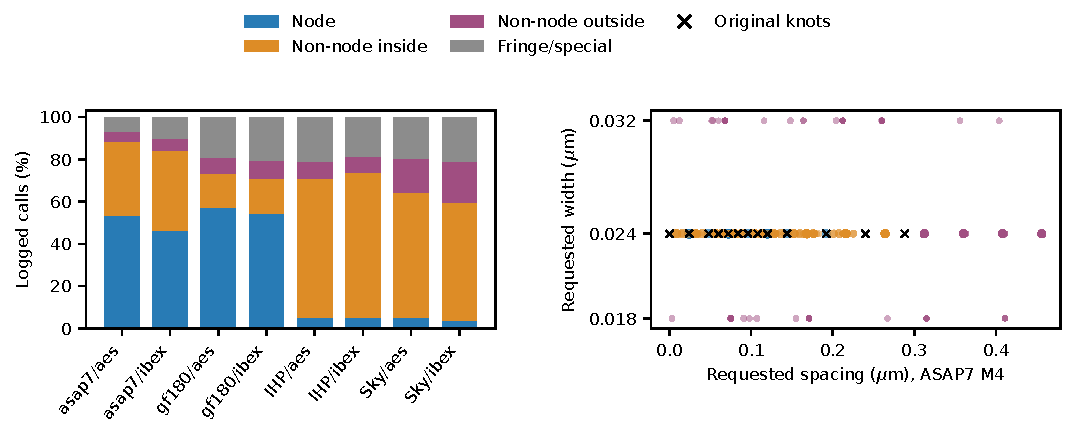
\includegraphics[width=\textwidth]{figures/query_census.pdf}
\caption{Measured non-node demand. Left: occurrence-weighted query classes over two logged capacitance getters on eight fixed layouts. Right: ASAP7 M4 requests and original knots; marker area reflects log occurrence. Counts exclude resistance, five-argument diagonal getters and later assembly; they are neither capacitance nor runtime weights. Raw and effective node identities differ under native mapping.}
\label{fig:census}
\end{figure*}

The trace preserves SPEF electrical records on all layouts. It establishes the frequency of non-node evaluation in these getters, not the fraction of all PEX work. Characterization holdout is a different quantity: it varies the available information rather than measuring runtime request frequency. We evaluate all four requested holdout levels without equating them to the census percentages.

\subsection{Problem formulation and kernel scope}
For context $c$, available observations $S=\{(x_i,y_i)\}$ and query coordinates $Q$, the estimator satisfies
\begin{equation}
\widehat y_Q=F_\theta(S,Q,c),\qquad \widehat y(x_i)=y_i\ (x_i\in S).
\end{equation}
An off-grid geometry need not lie outside support. Inside-support classification requires affine-space and hull membership; incompatible topologies or outputs are excluded explicitly. Only S values enter prediction; query reference values enter scoring.

The primary algorithmic comparison is the pinned OpenRCX finite-distance kernel and specified multilinear interpolation (MLI). Specified MLI implements the supplied xRC mathematical core. This comparison concerns the interpolation operator; commercial binaries and product-specific boundary policies are outside its scope. In $d$ dimensions,
\begin{equation}
\widehat y(x)=\sum_{\epsilon\in\{0,1\}^d}y_\epsilon
 \prod_{j=1}^d t_j^{\epsilon_j}(1-t_j)^{1-\epsilon_j}.
\end{equation}
Complete cells require $2^d$ vertices. Sparse-support completion and boundary clamping are separately declared extensions, not attributed to xRC. Physical data have rank one or two; four-dimensional evaluation is an implementation test only. OpenRCX comparison retains native width selection, integer geometry and four-unit compute bins; a continuous-distance variant isolates quantization effects. General numerical predictors are component controls.

\subsection{Related models and interfaces}
AttentionCap predicts capacitance matrices from conductor/material tokens~\cite{attentioncap}; Flash-CNNCap predicts window contributions in a three-dimensional DEF-to-SPEF workflow~\cite{flash}. Our component-supervised AttentionCap adaptation tests a specified observation budget and fitting recipe, rather than a general limit of matrix architectures. AttentionCap itself supports partial matrix-row supervision. Flash-CNNCap's 3D window task is not converted into a mismatched 2D speed ranking.

ResCap corrects initial physical estimates~\cite{rescap}; hybrid PEX selects extraction methods by window~\cite{hybrid}. Here the anchor uses current observations and fusion acts within a rule. CNPs~\cite{cnp} and attentive neural processes~\cite{anp} provide conditional regression interfaces. CNP is evaluated as such, not categorized as a field solver.

\section{Characterization-Conditioned Estimator}

\subsection{Support-derived anchor and representation}
The anchor $b_i(S,y_S)$ gives a stable estimate before learned correction. For rank-one support, it uses piecewise-linear interpolation with boundary clamping. For higher-rank support, it uses simplex interpolation inside the support hull and nearest-observation fallback outside it or for degenerate support. This support-derived anchor is distinct from the rank-matched multilinear baseline used in our comparisons.

Geometry tokens encode scaled coordinates, context, an observation indicator, available capacitance, and the anchor. The indicator distinguishes an unobserved zero placeholder from an observed zero. Context includes geometry family, layer indices, and available material descriptors; material tokens encode region bounds and permittivity. Coordinate and target scales are source-fitted and fixed at evaluation.

Binding positions to values distinguishes tables with similar geometry but different responses. The shared Transformer associates queries with relevant support and processes the full grid, including query--query interactions. Attention models relationships between observations and queries; its value relative to simpler regression is tested by the matched and conditional controls.

\subsection{Residual correction and component-wise fusion}
Let $h_i$ be the shared encoded representation and $\Delta^{\mathrm{NN}}_{i,k}$ its learned residual for component $k$. The final prediction is
\begin{equation}
\widehat y_{i,k}=\left[b_{i,k}+\sum_{e\in\mathcal E_i}\pi_{i,e,k}\Delta_{i,e,k}\right]_+,\quad i\in Q,
\label{eq:prediction}
\end{equation}
where $[z]_+=\max(z,0)$ and $\pi$ is normalized over applicable correction branches. The gate reads $h_i$ and support descriptors such as observation density, nearest-support distance, local span, and inside-support status. Its weights are component-specific, allowing ground and coupling responses to use different corrections at the same geometry.

\emph{Binary gate} combines zero correction with the raw neural residual. It therefore learns how far to move away from the support anchor. The \emph{Ungated residual} control adds the raw neural residual directly. \emph{Full fusion} augments the same interface with PCHIP where rank-one support permits it, aligned-width interpolation where applicable, six RBF-GP configurations, and a locally clamped reading of the neural residual. Each numerical branch contributes its prediction minus the anchor. The clamped neural reading restricts the completed value to the local support envelope inside support and retains the raw residual outside. The gate also receives component-wise correction disagreement descriptors. All applicable branches are evaluated before fusion; the gate combines outputs rather than skipping branch computation.

PCHIP supplies shape-preserving responses, aligned-width interpolation uses width slices, RBF kernels supply smooth alternatives, and neural corrections transfer cross-table relationships. GP length multipliers are $\{0.5,1,2\}$ times median nonzero support distance, paired with regularization $\{10^{-6},10^{-4}\}$. Unsupported branches are masked before gate normalization.

\subsection{Source training and rule export}
The encoder has two layers, four attention heads, and width 64; the gate hidden width is 32. Training samples tables and support masks with balanced geometry families and processes. Random, block, boundary, and eligible whole-width masks expose different support structures; holdout ratios are 10/30/50/70\%. A source-scaled Huber objective supervises withheld query components. Full, Binary, and Ungated use matched source pools, residual initialization, samplers, optimizer settings, update counts, and three training seeds. AdamW uses learning rate $2\!\times\!10^{-4}$ and weight decay $10^{-4}$. Table~\ref{tab:data} lists update counts; completion predictions average three members.

We restore $y_S$ exactly and write query predictions to their original capacitance fields, preserving other fields including resistance. OpenRCX consumes the completed rules on the fixed routed database; STA uses identical libraries and constraints. Learning thus enters offline rule construction while retaining native layout processing.

\subsection{Populating the native evaluation structure}

\begin{figure*}[t]
\centering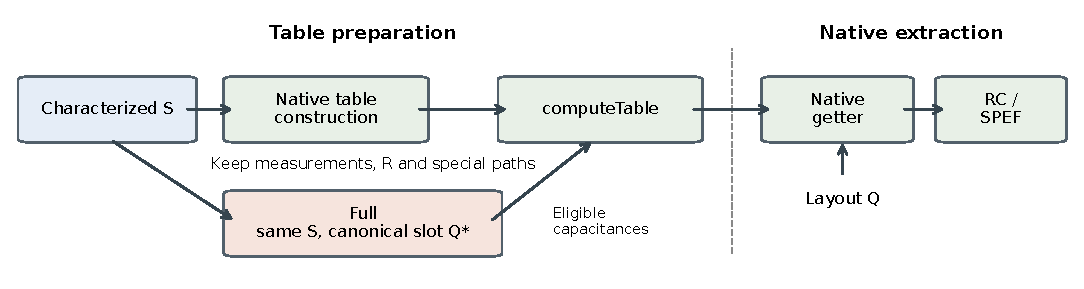
\includegraphics[width=\textwidth]{figures/compute_table_interface.pdf}
\caption{Learning populates eligible internal capacitance slots during preparation. The original constructor supplies the complete native table; the hook changes only covered coupling/fringe values. Real observations, resistance and special returns remain native. Layout queries retain the original getter and RC assembly.}\label{fig:interface}
\end{figure*}
Figure~\ref{fig:interface} separates preparation from native queries. The preparation hook runs immediately after OpenRCX constructs a distance compute table and before getters use it. Keys include process/corner, rule/configuration identity, family, layers, mapped width, slot index, represented separation, output components and units. Predictions are evaluated at the coordinate represented by the slot, not at an arbitrary raw request. All S values remain real observations; generated values are never fed back as support.

The evaluated scope is finite, non-sentinel OVER/UNDER/OVERUNDER tables with uniquely matched source-held-out rules. Measurement-bin collisions, special tails, unsupported paths and resistance remain native. Boundary paths that return the measure table are preserved. Only coupling and fringe compute fields are written. Full-grid preparation uses deterministic coordinate order and Q chunks of 32; no query-dependent Transformer support states are cached.

We compare unmodified extraction, interface-disabled extraction, native-value pass-through, Binary and Full injection. A separate trace build checks getter values; the release build leaves getter bodies unchanged. Inventories must match across both designs of each process before claiming design-independent grid reuse. The pinned public API defers loading until extraction, so the first inventory extraction is charged to preparation. This is explicit measured overhead, not a free rule-only operation.


\section{Experimental Setup}
\subsection{Data and evaluation populations}
\begin{table}[t]
\centering\caption{Data and source-training opportunities. Counts are fitting/selection/confirmation tables. Public inventory size is 1,713; k denotes 1,000 updates. Matched = Full/Binary/Ungated joint training.}
\label{tab:data}
\small\setlength{\tabcolsep}{3pt}
\begin{tabular}{lccc}\toprule
 & Public & FEM & Transfer\\\midrule
Geometry rank & 1 & 2 & 2\\
Components & coupling, ground & \multicolumn{2}{c}{lateral, ground, diagonal}\\
Units & native/length & F/m & F/m\\
Fit/select/confirm & 1051/246/340 & 16/24/16 & 8/12/8\\
Fit/confirm nodes & variable & 153/128 & 153/128\\
Budgeted tables & 338 & 16 & 8\\
Matched updates & 24k & 12k & 12k\\
MLP/CNP updates & 3k & 3k & 3k\\
Adapted AC updates & -- & 3k & 3k\\\bottomrule
\end{tabular}
\end{table}
Table~\ref{tab:data} distinguishes the public rule library from FEM references for two-dimensional cross sections with width and spacing variation. FEM covers FreePDK15 and ASAP7; cross-process prediction trains and selects on FreePDK15 and evaluates on ASAP7. Target observations are inputs but target queries are excluded from training and selection. The public confirmation view and native holdout are separately defined evaluation populations. All 84 native holdout tables are excluded from public fitting and selection.

\emph{Controlled characterization subsampling} evaluates 30\% random, block, and boundary masks, partitioning queries into inside- and outside-support conditions. We retain the original method-specific mask sequences and score aggregation. \emph{Characterization-support-size sensitivity} seal a common evaluation subset of approximately 20\% of each table, then reveal geometries in farthest-first coverage order. Three data seeds (11, 29, 47) define paired populations across methods and budgets. The initial four observations count toward $B$. Public tables support $B=4,8$; FEM and transfer support $B=4,8,16,32,64$. Each geometry query returns all output components. Short tables use a separate feasible two-observation protocol and are excluded from the main budget curves.

\subsection{Comparators and training opportunities}
Numerical controls include Anchor, rank-matched multilinear interpolation (CMI), piecewise-linear interpolation, PCHIP, inverse-distance weighting, RBF-GP, and local affine fitting. CMI combines complete-cell multilinear interpolation with support-only sparse completion and clamping. Its extensions are distinct from the specified complete-cell core and are not attributed to a commercial implementation. Controlled-subsampling GP uses its specified median-distance kernel; budgeted GP selects from the six configurations on source validation. Affine neighborhoods are validation-selected: four public or eight FEM points.

The budgeted learning controls comprise a geometry/context MLP, a mean-context CNP, and adapted AttentionCap. MLP/CNP select their source learning rate from $10^{-3}$ and $3\!\times\!10^{-4}$ on source validation. The MLP then takes 200 target fitting steps using only $S$, selected from 0/50/200; CNP conditions on $S$ without parameter updates. Adapted AttentionCap retains the official Transformer/symmetric matrix head~\cite{attentioncode}, converts recorded conductor rectangles and materials to tokens with an external-boundary token, and supervises only the same three FEM components. Its 50 target fitting steps are source-validation-selected from the same candidates. There is no public-rule AttentionCap result because the required matrix geometry representation is not defined for those inputs. Equal target observations therefore do not imply equal source-training compute; the matched architectural comparison is Full/Binary/Ungated.

\begin{table*}[!t]
\centering\caption{Controlled characterization subsampling at 30\%: mean-mask macro NRMSE (lower is better). In/Out denote geometric support; Boundary is the boundary-extrapolation mask. All 15 conditions are shown. Full, Binary, and Ungated average three matched members' predictions. Bold is best among displayed methods. The controlled-subsampling GP uses its specified kernel; the budget-selected GP in Fig.~\ref{fig:budget} is a separate comparison.}
\label{tab:missing}
\small\setlength{\tabcolsep}{6pt}\begin{tabular}{llrrrrrrr}
\toprule
Data & Queries & CMI & Anchor & Affine & RBF-GP & Ungated & Binary & Full \\
\midrule
Public & In/random & 0.1286 & 0.1286 & 0.2062 & 0.4011 & 0.0875 & 0.0850 & \textbf{0.0803} \\
Public & In/block & 0.2812 & 0.2812 & 0.4324 & 0.2490 & \textbf{0.0645} & 0.0701 & 0.0678 \\
Public & Out/random & 0.5531 & 0.5531 & 0.4766 & 0.9120 & 0.0965 & 0.0954 & \textbf{0.0910} \\
Public & Out/block & 0.9546 & 0.9546 & 0.5588 & 3.5596 & 0.1455 & 0.1420 & \textbf{0.1391} \\
Public & Boundary & 1.1867 & 1.1867 & 0.6503 & 4.6800 & 0.1675 & 0.1629 & \textbf{0.1620} \\
FEM & In/random & 0.0495 & 0.0208 & 0.0389 & 0.0116 & 0.0529 & 0.0387 & \textbf{0.0103} \\
FEM & In/block & 0.1502 & 0.1286 & 0.1579 & 2.8414 & 0.0885 & 0.0560 & \textbf{0.0366} \\
FEM & Out/random & 0.1344 & \textbf{0.0606} & 0.0621 & 1.0237 & 0.1336 & 0.1303 & 0.0895 \\
FEM & Out/block & 0.9790 & 0.6542 & 0.3374 & 18.3431 & 0.1867 & 0.1479 & \textbf{0.1203} \\
FEM & Boundary & 0.6404 & 0.5663 & 0.2376 & 17.6758 & 0.1761 & 0.1388 & \textbf{0.1137} \\
Transfer & In/random & 0.0488 & 0.0205 & 0.0381 & \textbf{0.0113} & 0.0588 & 0.0432 & 0.0159 \\
Transfer & In/block & 0.1473 & 0.1246 & 0.1542 & 2.5309 & 0.0868 & 0.0640 & \textbf{0.0531} \\
Transfer & Out/random & 0.1330 & 0.0595 & \textbf{0.0594} & 0.8194 & 0.1172 & 0.1124 & 0.0877 \\
Transfer & Out/block & 0.9583 & 0.6374 & 0.3288 & 16.0145 & 0.1482 & \textbf{0.1291} & 0.1358 \\
Transfer & Boundary & 0.6297 & 0.5580 & 0.2364 & 15.5718 & 0.1172 & \textbf{0.1037} & 0.1073 \\
\bottomrule
\end{tabular}

\end{table*}
\subsection{Metrics and native reference}
For a component group $g$, the common error quantity is
\begin{equation}
E_g=\sqrt{\frac{\sum_{i\in Q_g}(\widehat y_i-y_i)^2}{\sum_{i\in Q_g}y_i^2}}.
\label{eq:metric}
\end{equation}
Zero-truth-energy groups are excluded from normalized error and retained for absolute-error reporting. Controlled-subsampling \emph{mean-mask macro NRMSE} pools squared errors within each process/family/component and mask, takes the macro mean, then averages masks. Fixed-budget \emph{pooled-replicate macro NRMSE} pools data seeds before the ratio and square root, then takes the group macro. The support-protocol analysis instead uses \emph{mean-member, group-balanced NRMSE}: component means within tables, averaging data seeds and tables within process/layer groups, then groups and budgets equally, before averaging member scores. It does not average member predictions first.

Native evaluation uses AES and Ibex on ASAP7, GF180, IHP SG13G2, and Sky130HS: eight fixed layouts. The reference is full-rule extraction on the same routed database, libraries, constraints, and tools. Controlled-subsampling exports use block masks at 30/50\%; net-C NRMSE is averaged over three seeds, while WS/TNS report the maximum absolute deviation over those seeds. Fixed-budget exports use $B=4,8$ and three data seeds, replacing 83 eligible held-out tables in otherwise complete libraries. One two-node ASAP7 OVER table retains complete values under the common feasibility rule. Fixed-budget metrics average seeds within each layout--budget condition. P99 is the within-run 99th percentile of absolute finite-endpoint slack errors, subsequently seed-averaged. All timing errors are relative to the full-rule reference.

\begin{figure*}[!t]
\centering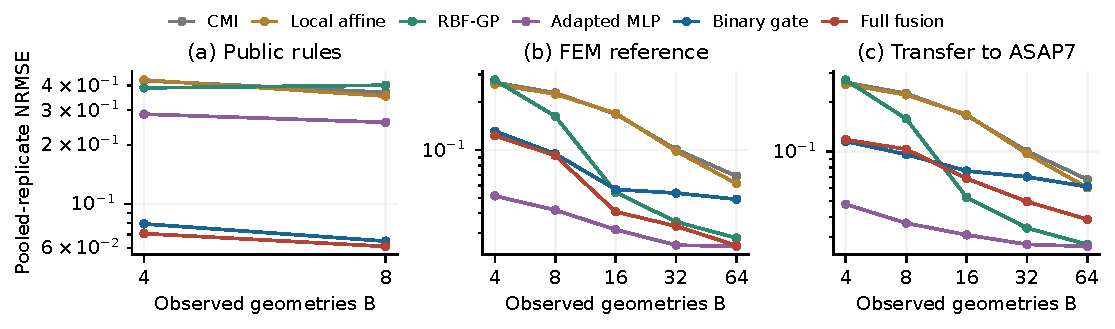
\includegraphics[width=\textwidth]{figures/budget_accuracy.pdf}
\caption{Fixed-observation-budget completion: pooled-replicate macro NRMSE on common sealed queries, with three data seeds and three-member learned ensembles. All displayed methods use the same $B$ target geometries. MLP fits to those observations; Full/Binary keep learned parameters fixed. Only feasible budgets are plotted. CNP, Ungated, and adapted AttentionCap are reported in Table~\ref{tab:aux}.}
\label{fig:budget}
\end{figure*}
\section{Results}
\subsection{Controlled characterization subsampling}

Full fusion improves over CMI in all 15 conditions and Binary in 13 (Table~\ref{tab:missing}). Across all five FEM conditions, its numerical corrections add value: NRMSE falls from 0.0387 to 0.0103 for in-support random queries and from 0.0560 to 0.0366 for blocks. Relative reductions range from 18.1--73.3\%\unskip, supporting the correction bank under these coverage patterns.

Public architecture gaps are smaller. Full reaches 0.0803/0.0678 on in-support random/block queries versus Binary's 0.0850/0.0701; Ungated is better on blocks (0.0645). Full reduces out-of-support block and boundary errors to 0.1391 and 0.1620. Cross-table residual learning helps substantially over multilinear completion even where gate complexity has modest benefit.

Cross-process prediction with fixed learned parameters achieves 0.0159 for in-support random queries, compared with Binary's 0.0432. Full also improves over Binary on in-support blocks and out-of-support random queries; Binary is better on out-of-support blocks and the boundary condition. Local affine fitting is a strong numerical counterexample: it obtains 0.0621 versus Full's 0.0895 on FEM out-of-support random queries and 0.0594 versus 0.0877 on transfer. The support anchor is also competitive there. Geometry outside the observed hull therefore does not by itself identify a setting requiring learned fusion.

\begin{figure*}[!t]
\centering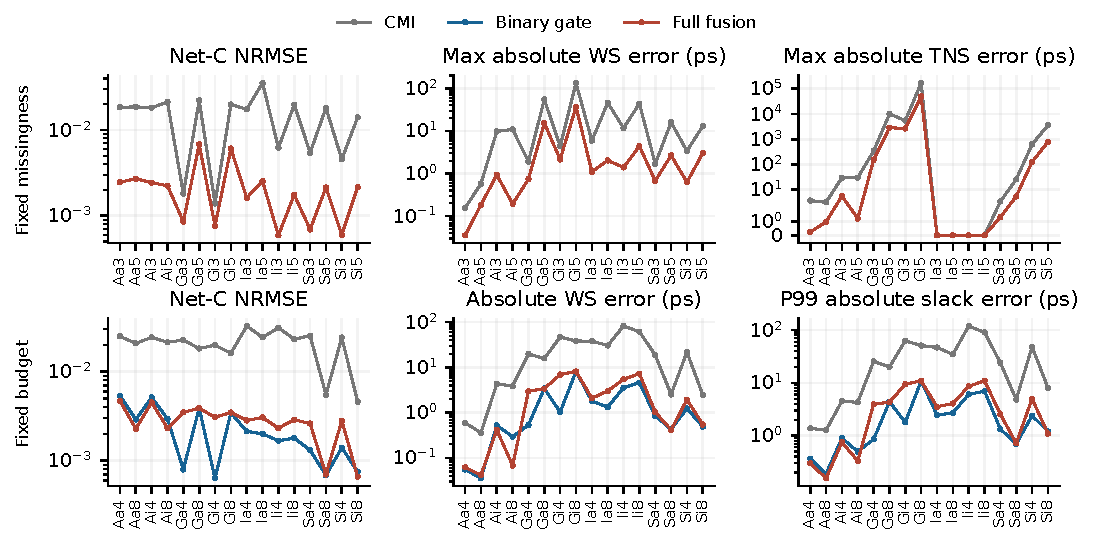
\includegraphics[width=\textwidth]{figures/native_fidelity.pdf}
\caption{Native fidelity for every layout and condition. A/G/I/S: ASAP7/GF180/IHP/Sky130HS; a/i: AES/Ibex. Top: 30/50\% block holdout (suffix 3/5); net-C is seed-mean NRMSE, WS/TNS are maximum absolute deviations over three seeds. Bottom: budgets 4/8; all values are three-seed means. P99 is absolute endpoint-slack error within each run. Timing units are ps; the top-right TNS axis uses a symmetric-log scale to retain exact zeros. Lines connect conditions for readability, not a geometry sweep. The two rows have different aggregation and are compared only within their own protocol.}
\label{fig:native}
\end{figure*}
\subsection{Fixed-observation-budget comparison}

Figure~\ref{fig:budget} separates observation count from the holdout patterns above. On public rules, Full obtains 0.0708 at $B=4$ and 0.0609 at $B=8$, compared with Binary's 0.0793/0.0648 and adapted MLP's 0.2860/0.2599. The conditional residual representation performs well using sparse table-specific observations without target parameter updates.

FEM yields a different comparison. At $B=4$, adapted MLP obtains 0.0515 versus Full's 0.1233 and Binary's 0.1315. At $B=64$, Full (0.0250), selected GP (0.0280), and adapted MLP (0.0248) are close. In transfer at $B=64$, GP and adapted MLP reach 0.0271 and 0.0264, respectively, compared with Full's 0.0386. The availability of a reusable source-trained representation thus does not eliminate the benefit of fitting a simple predictor to target observations.

\begin{table}[t]
\centering\caption{Additional fixed-budget controls, pooled-replicate macro NRMSE. AC denotes component-supervised adapted AttentionCap. Dashes mark unavailable or infeasible evaluations. These AC results evaluate the stated rule-completion adaptation, rather than rank the original capacitance-matrix task.}
\label{tab:aux}\small\setlength{\tabcolsep}{2pt}\begin{tabular}{llrrrrr}
\toprule
Data & Method & 4 & 8 & 16 & 32 & 64 \\
\midrule
Public & Ungated & 0.0776 & 0.0682 & -- & -- & -- \\
Public & CNP & 0.2650 & 0.2374 & -- & -- & -- \\
Public & Adapted AC & -- & -- & -- & -- & -- \\
FEM & Ungated & 0.1100 & 0.0917 & 0.0681 & 0.0657 & 0.0609 \\
FEM & CNP & 0.2356 & 0.2313 & 0.2297 & 0.2274 & 0.2271 \\
FEM & Adapted AC & 0.4546 & 0.2256 & 0.2025 & 0.1677 & 0.1657 \\
Transfer & Ungated & 0.1410 & 0.1282 & 0.1069 & 0.0954 & 0.0814 \\
Transfer & CNP & 0.2138 & 0.2126 & 0.2135 & 0.2127 & 0.2136 \\
Transfer & Adapted AC & 6.8753 & 0.3199 & 0.2120 & 0.2153 & 0.1791 \\
\bottomrule
\end{tabular}

\end{table}
Table~\ref{tab:aux} retains CNP and adapted AttentionCap. CNP is less accurate than Full/Binary in these cohorts. Adapted AttentionCap improves from 0.4546 at FEM $B=4$ to 0.1657 at $B=64$, but reaches 6.8753 at transfer $B=4$, showing sensitivity to sparse component-supervised fitting. In a separate reverse-direction MLP experiment (ASAP7 to FreePDK15), target fitting reduces NRMSE from 0.4414 without updates to 0.0569 at $B=4$ and 0.0284 at $B=64$.

Target fitting consumes updates per table; Full/Binary reuse weights. Full still evaluates its numerical bank: recorded shared encoding plus one forward pass costs 15.05--18.01\,ms for Full-L versus 8.58--10.75\,ms for Binary-L across the support-analysis budgets (single-member component costs, not ensemble wall times). FEM characterization work replays recorded costs including initial support; public accesses are simulated. Several strong methods meet the evaluated source-validation tolerances at the first tested $B=4$. These minimum-budget results are retrospective comparisons, not deployment stopping rules with access to query truth.

\subsection{Native extraction and timing fidelity}

Figure~\ref{fig:native} connects table completion to downstream electrical quantities. Under controlled subsampling, Full improves net-C fidelity and reduces worst-slack absolute error relative to multilinear completion in all 16 layout--holdout conditions. For GF180 Ibex at 50\% holdout, net-C NRMSE is 0.0061 versus 0.0199, while maximum absolute worst-slack error is 37.01 versus 132.8\,ps. The maximum absolute TNS deviation decreases from 168.6 to 50.22\,ns. Zero TNS deviations on IHP coexist with changes in positive worst slack, motivating the separate timing columns.

Under fixed observation budgets, Full improves net-C and worst-slack fidelity over CMI in all 16 layout--budget conditions. Relative to Binary, its net-C error improves in six conditions and its worst-slack error improves in four. Binary has lower P99 absolute endpoint-slack error in ten conditions. The largest Full-minus-Binary P99 difference is $+7.6433$\,ps for GF180 Ibex at $B=4$, an increase in prediction error relative to the complete-rule reference.

Equal-layout averages also favor Binary over Full at $B=4$: net-C NRMSE is 0.002309 versus 0.003297, absolute worst-slack error is 1.1989 versus 2.6146\,ps, and P99 absolute slack error is 2.0092 versus 4.2546\,ps. CMI's mean worst-slack error is 29.0093\,ps. Gains over multilinear completion propagate to timing, while the extra fusion bank has more selective benefit.

Tail and decision metrics provide a further distinction. Against Binary, Full improves/ties/worsens absolute TNS error in 5/4/7 conditions, ties false negatives in all 16, and ties/worsens false positives in 14/2. Against CMI, TNS counts are 13/3/0, while false positives improve/tie/worsen in 4/9/3. All comparisons use the same completed-table population and fixed designs. Native fidelity is agreement with full-rule extraction; shared libraries and layouts make these conditions dependent, and the sensitivity of a circuit path can amplify errors that appear small at the table level.

\subsection{Support-protocol sensitivity and computational tradeoffs}
\begin{figure}[t]
\centering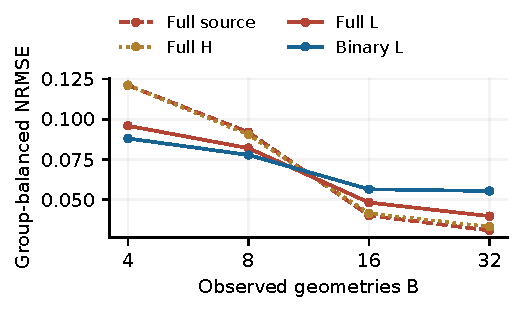
\includegraphics[width=\columnwidth]{figures/support_protocol.pdf}
\caption{Support-protocol sensitivity: mean-member, group-balanced NRMSE, averaged over three training seeds. Source denotes the source-trained Full; H and L use 2,000 matched continuation steps per member. Binary-L is better at $B=4,8$ on average. Full-L exceeds Binary-L at $B=16,32$ but is less accurate than source-trained Full at those budgets. This metric differs from the ensemble metric in Fig.~\ref{fig:budget}.}
\label{fig:support}
\end{figure}
The 153-node FEM training tables retain at least 46 observations under 10/30/50/70\% holdout; whole-width holdouts also retain more than four. To study the low-budget mismatch, we compare Full/Binary under original support (H) and low-budget support (L), using common source data, three original seeds, paired episodes, and 2,000 continuation steps per endpoint (12 total). L uses coverage sampling at $B=4,8,16,32$, changing support count and coverage jointly.

Figure~\ref{fig:support} shows the resulting interaction. The H-minus-L mean error improvement is 0.005066 for Full and 0.015766 for Binary; their difference is $-0.010701$, indicating a larger response for Binary. Full-L retains a four-budget average advantage of 0.002939 over Binary-L, with the same sign for all three seed-level averages. At $B=4$, however, Binary-L wins for all three seeds; at $B=8$, it wins for two. At $B=16,32$, Full-L is better than Binary-L but worse than both source-trained Full and Full-H. Relative to source-trained Full, its mean errors increase by 20.0\% and 28.9\% at those budgets.

Original-support retention error increases from 0.04359 to 0.05209 for source-trained Full versus Full-L, and from 0.06366 to 0.06808 for Binary. Full's four-budget advantage over Binary narrows from 0.014088 to 0.002939: low-budget continuation primarily closes the gap for the simpler gate, with a denser-support accuracy cost. Across 1,728 paired component/seed/cell outcomes, Full-L's capacitance P99 error is lower/tied/higher than Binary-L in 887/225/616 cases. These correlated rule-level tails are separate from the native STA tails.


\subsection{Native queries and independent template references}
We instrument two capacitance getters in OpenROAD
\texttt{0b54bb3203}: finite width/distance evaluation and indexed fringe lookup.
Original and instrumented extraction produce identical SPEF electrical records
on all eight fixed routed databases. Across 9,888,586 logged calls and 19,562
unique rule/geometry keys, 2,696,515 calls hit characterization nodes,
4,547,424 are non-node queries within the selected width slice's support,
and 967,755 lie outside it. The remaining 1,676,892 are fringe/special calls.
Non-node calls represent 55.77\% of this denominator and 67.16\% of finite
distance calls. The trace excludes resistance, five-argument diagonal getters,
and subsequent assembly; it is not a count of every extraction operation.



OpenRCX maps widths and constructs an internal distance compute grid.
Among raw non-node calls, 849,663 return an effective characterization node;
these are reported as quantized-to-node, separately from interpolation.
An independent reproduction of the finite, non-sentinel computation matches
29,735 design-specific query records (8,211,694 occurrences), with maximum
support-scaled difference $2.1\times10^{-16}$. Rule identity is uniquely
resolved for 95.42\% of logged calls. This is an interface identity result;
matching rule names does not establish matching electrostatic materials.

\begin{table}[t]
\centering\caption{Off-grid query comparisons, macro NRMSE. Native agreement: 480 queries from 42 source-held-out rule groups, using every supplied rule sample and actual OpenRCX returns as reference. FEM: 71 independent template queries with 153 matched support samples per context. Weighted FEM uses occurrence counts divided by sampling probability. Native agreement and direct physical error have different references and units; compare methods only within a column.}
\label{tab:offgrid}\scriptsize\setlength{\tabcolsep}{2pt}\begin{tabular}{lrrr}\toprule
Method & Native agreement & FEM unique & FEM weighted\\\midrule
Multilinear & 0.00761 & 0.00452 & 0.00527\\
Support anchor & 0.00761 & 0.00451 & 0.00527\\
Local affine & 0.17500 & 0.05254 & 0.05915\\
RBF-GP & 0.41736 & 0.05371 & 0.04158\\
Ungated & 0.21853 & 0.02688 & 0.02309\\
Binary & 0.24363 & 0.02218 & 0.02323\\
Full & 0.23620 & 0.01675 & 0.01456\\
Adapted MLP & 0.34070 & 0.01889 & 0.01792\\
CNP & 0.24988 & 0.16575 & 0.17161\\
\bottomrule\end{tabular}
\end{table}

For direct reference evaluation, 114 geometry candidates arise from ASAP7 AES
and Ibex calls on M4/M5 with adjacent OVER, UNDER, and OVERUNDER contexts.
They account for 86,587 calls (0.876\% of the logged denominator).
Geometry-only, hash-ordered stratification fixes 12 pilot and 71 formal queries
before solving or inspecting errors. Each query is absent from the original
CTF characterization nodes at database resolution. Widths are 0.024 or
0.032\,$\mu$m. All 153 original samples in each of six contexts remain available;
no characterization node is masked to create these queries.

The physical cohort is a \emph{layout-parameterized template}: logged width
and spacing drive symmetric, equal-width side wires, finite adjacent grounded
planes, and an exterior grounded boundary in the declared ASAP7 CTF stack.
It does not retain arbitrary asymmetric routing, net connections, or a full
layout section. Ground and summed lateral coupling are projected from the
Maxwell matrix in F/m. Original native calibration materials and projections
are not jointly aligned with this template, so no native-versus-FEM physical
accuracy claim is made. For the same template, direct P2 FEM solves provide
query labels independently of prediction; support geometry, solver hashes,
and component projections are verified against the reused matrices.

All 83 pilot/formal geometries pass coarse/fine/doubled-domain checks and
component-scaled convergence limits. Twelve additional on-grid controls
reproduce the reused matrices exactly. Macro normalized component uncertainty
is 0.00016, compared with Anchor/Full/Binary errors of
0.00451/0.01675/0.02218. Source training and selection for this cohort use
FreePDK15 only. Table~\ref{tab:offgrid} shows that the support anchor is more
accurate than learned correction with the full supplied characterization.
Full improves over Binary and adapted MLP on this cohort, but does not improve
on numerical interpolation. In native replay, interpolation also agrees more
closely with OpenRCX than the learned methods. Agreement alone does not rank
physical accuracy.

Queries are sorted by geometry hash within a rule context and processed in
chunks of at most 32 with all support samples. Original-grid API outputs and
support restoration are bit-exact. Development checks show that changing
query sets changes Full's predictions (maximum 0.0205 in source-normalized
units in the public check), while fixed-policy input reordering leaves them
unchanged. Raw token reordering in FEM changes Full by up to 0.00319 in source-normalized units; support envelope and gate descriptors change even when token features and anchor values are unchanged. Canonicalization is therefore part of the protocol. This is batch-conditioned query evaluation.

\begin{figure*}[t]
\centering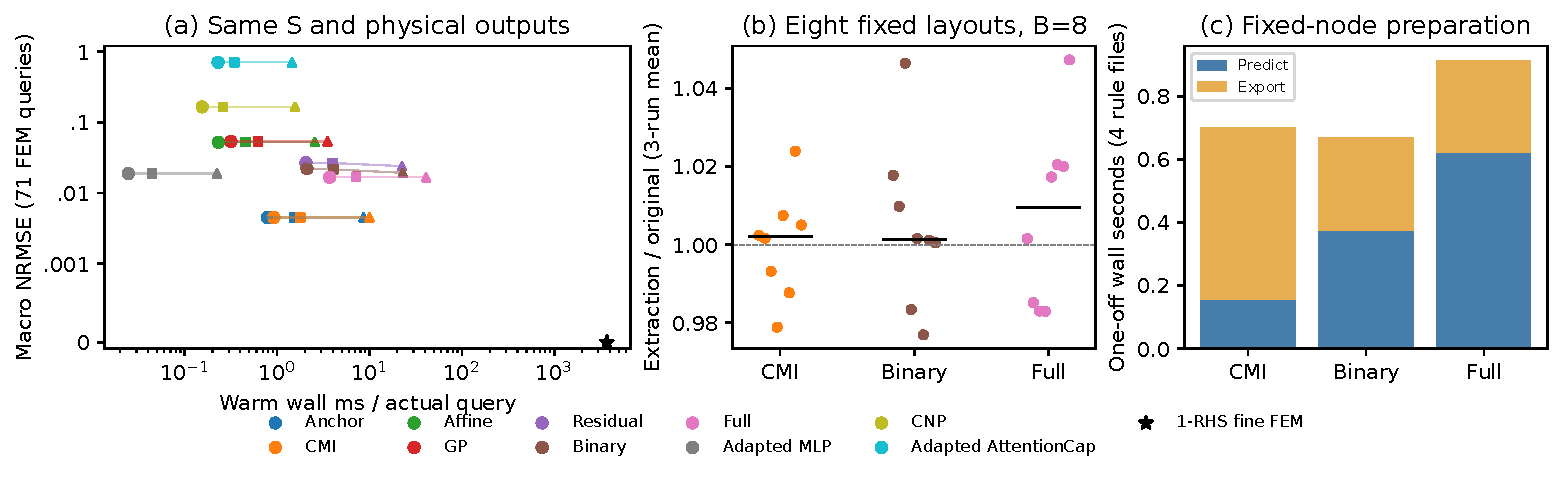
\includegraphics[width=\textwidth]{figures/runtime_accuracy.pdf}
\caption{Accuracy and deployment cost. (a) Same 71 template queries: circles/squares/triangles use Q limits 32/8/1, respectively; each point has its own precision measurement. The ordinate is linear below 0.001 and logarithmic above it. The fine-solver marker denotes numerical agreement with the certified fine reference, not zero discretization error. Adaptation/loading is separate from warm evaluation. (b) Per-layout mean extraction ratios over three release runs; bars mark medians across eight layouts. (c) One-off prediction and fixed-node export for four process libraries at B=8, seed 11, excluding separately reported shared loading/support preparation. This panel uses its own controlled-support protocol, not the accuracy population in (a).}
\label{fig:runtime}
\end{figure*}

% BEGIN RUNTIME_ADDENDUM
\subsection{Accuracy--Runtime Trade-offs and Deployment Cost}
We measure the same queries on one pinned Xeon Gold 6530 CPU thread,
with three warmups and 20 randomized timing blocks. Each batch limit
$Q\in\{1,8,32\}$ has separately evaluated predictions. Times include
query encoding, numerical candidates, all three ensemble members, and output
assembly; support and material tokens are excluded from the query denominator.
Table~\ref{tab:offgrid} and Fig.~\ref{fig:runtime} pair error with measured cost.
For the 71 templates, Full's warm amortized cost is
3.706\,ms/query, versus 2.110 for Binary
and 0.788 for Anchor. Full's actual single-request mean
is 40.97\,ms; throughput does not imply this latency.

Retaining each fixed-support fit reduces adapted MLP's warm cost to
0.025\,ms/query, with NRMSE 0.01889;
its one-time six-context fit costs 14.03\,s,
including first-use optimizer initialization. Adapted AttentionCap costs
0.230\,ms/query but has NRMSE 0.70695
on these same templates; its source-selected adaptation costs
11.27\,s. No query labels enter either fit.
Transformer support states are not cached: changing $Q$ changes its predictions.
Anchor/CMI remain more accurate than Full with this full support.

A resident one-RHS P2 solve takes 3.719\,s/query,
including a regenerated fine mesh, assembly, factorization and both nonzero
outputs. Three passes match the certified full-matrix target row within
1.5e-15 relative scale. Cold fine-only solving and
three-level certification cost 316.1 and
799.1\,s over these 71 geometries, respectively.
Surrogate errors exceed reference uncertainty; these are not equal-accuracy
speedup claims.

For native agreement, a validated C++ finite-distance getter counterpart takes
1.72\,ns/query in long warm loops after width/context resolution;
the ctypes calling loop takes 0.567\,$\mu$s/query.
Neither measures a complete PEX query. In 96 release-OpenROAD runs (eight
unchanged layouts, four rule variants, three repeats), Full's extraction-time
ratio to original rules ranges from 0.983 to 1.047.
At $B=8$, seed 11, prediction and export for all four libraries cost
0.70/0.67/0.91\,s for CMI/Binary/Full,
plus shared input, support and model loading. Each library serves two measured
designs. SPEF writing and STA are timed separately; rule parsing remains in
extraction. The exported electrical results match the frozen variants exactly.
This configuration keeps learned inference outside the native extraction loop;
it establishes neither added-node enrichment nor online model replacement.
% END RUNTIME_ADDENDUM
\begin{table*}[t]
\centering\caption{CPU query timing on the same 71 FEM templates. Warm ms/Q uses actual batch sizes with a maximum of 32; Q=1 mean/P95 are measured request latencies in ms. Fit is the one-time total for six support contexts, including first-use optimizer initialization. All neural results use three members; loading is reported separately. Complete component MAE/P95/P99 and per-block variation are in the reproduction CSVs.}
\label{tab:runtime_detail}\small\begin{tabular}{lrrrrr}\toprule
Method & NRMSE & ms/Q & Q=1 mean & Q=1 P95 & Fit (s)\\\midrule
Multilinear & 0.00452 & 0.923 & 10.008 & 10.672 & 0.00\\
Support anchor & 0.00451 & 0.788 & 8.643 & 8.971 & 0.00\\
Local affine & 0.05254 & 0.232 & 2.558 & 2.650 & 0.00\\
RBF-GP & 0.05371 & 0.316 & 3.516 & 3.604 & 0.00\\
Ungated & 0.02688 & 2.051 & 22.511 & 23.969 & 0.00\\
Binary & 0.02218 & 2.110 & 22.971 & 24.383 & 0.00\\
Full & 0.01675 & 3.706 & 40.973 & 44.127 & 0.00\\
Adapted MLP & 0.01889 & 0.025 & 0.222 & 0.259 & 14.03\\
CNP & 0.16575 & 0.155 & 1.561 & 1.767 & 0.00\\
Adapted AC & 0.70695 & 0.230 & 1.454 & 1.532 & 11.27\\
\bottomrule\end{tabular}

\end{table*}
\begin{figure*}[t]
\centering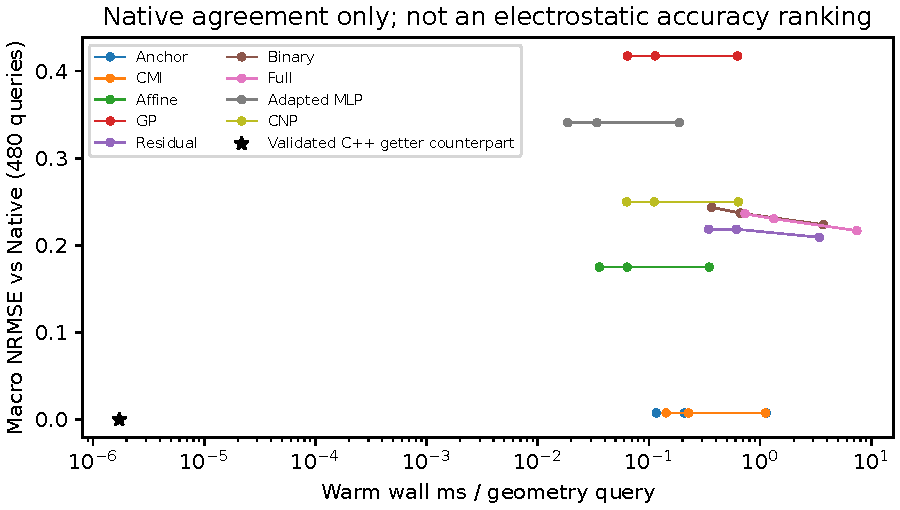
\includegraphics[width=.8\textwidth]{figures/runtime_native_agreement.pdf}
\caption{Separate native-agreement runtime comparison on all 480 queries. Each method has independently scored Q limits 1, 8 and 32. The validated C++ counterpart reproduces the reference by construction, after width/context resolution. This is interface agreement, not a physical error ranking.}
\label{fig:runtime_native}
\end{figure*}


\subsection{Discussion}
Target observations support three deployment choices: numerical fitting, source-trained conditional residuals, and target parameter adaptation. Full fusion adds value in all five FEM controlled-subsampling conditions; sparse support and native timing tails favor simpler alternatives in several comparisons. With all supplied characterization samples, interpolation is more accurate on the layout-parameterized template cohort. Query-level replay, offline addition of rule nodes, and in-extractor replacement are distinct deployment levels. The evidence supports query replay, fixed-node rule export and the separate internal compute-table injection evaluated below. Neural inference occurs during preparation; runtime getters remain native.

Public geometry is rank one, FEM models idealized two-dimensional cross sections, and native exports replace held-out tables within otherwise complete libraries. Budgeted learning controls have different source-training opportunities; their controlled-subsampling counterparts use distinct protocols. The support analysis covers four process/layer groups and three seeds, changing count and coverage jointly. Deployment selection should consider table accuracy, target fitting, correction-bank computation, and downstream error metrics.


\begin{figure*}[t]
\centering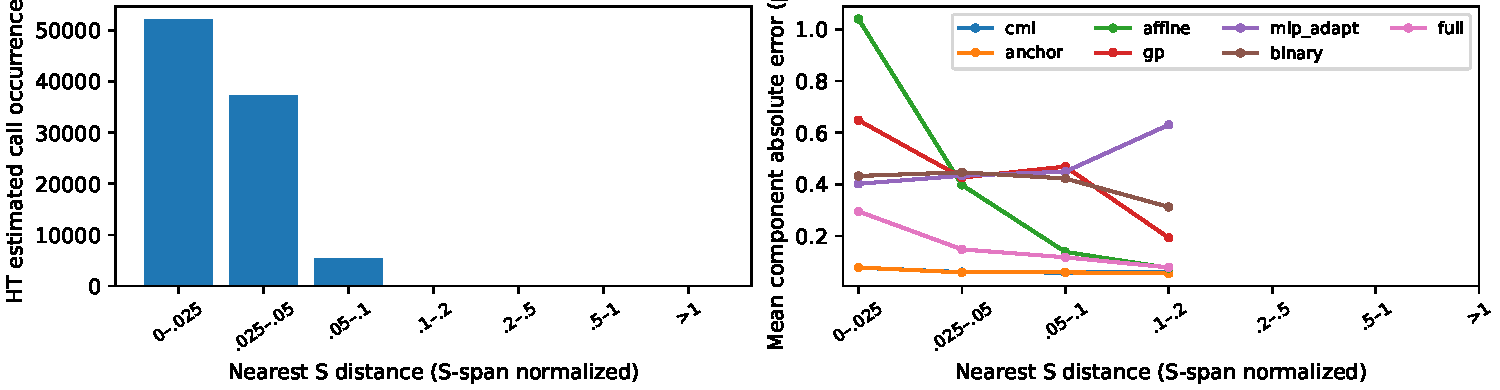
\includegraphics[width=\textwidth]{figures/query_errors.pdf}
\caption{Occurrence and error versus S-only normalized nearest-support distance. Fixed bins are shared by all methods; the direct reference is the declared template, not an exact layout section. Occurrence estimates use inverse inclusion probabilities.}
\end{figure*}
\clearpage
\section{Production Kernels and Internal Compute-Table Deployment}
\subsection{Coverage sensitivity over all four holdouts}
Figure~\ref{fig:coverage} includes all 60 domain--holdout--condition cells. Full has lower error than the OpenRCX kernel, MLI with the explicit extension, and Binary in 60, 60, and 49 cells, respectively. The kernels share 21,840/21,840 feasible support/query episodes. Complete MLI cells cover 20.7\% of requested queries across the sweep; the remainder use the declared boundary or sparse-support extension. The inventory flags 11,245 repeated rounded S/Q episodes rather than treating them as additional independent evidence. Detailed cells and all numerical controls are retained in the expanded tables.

\begin{figure*}[t]\centering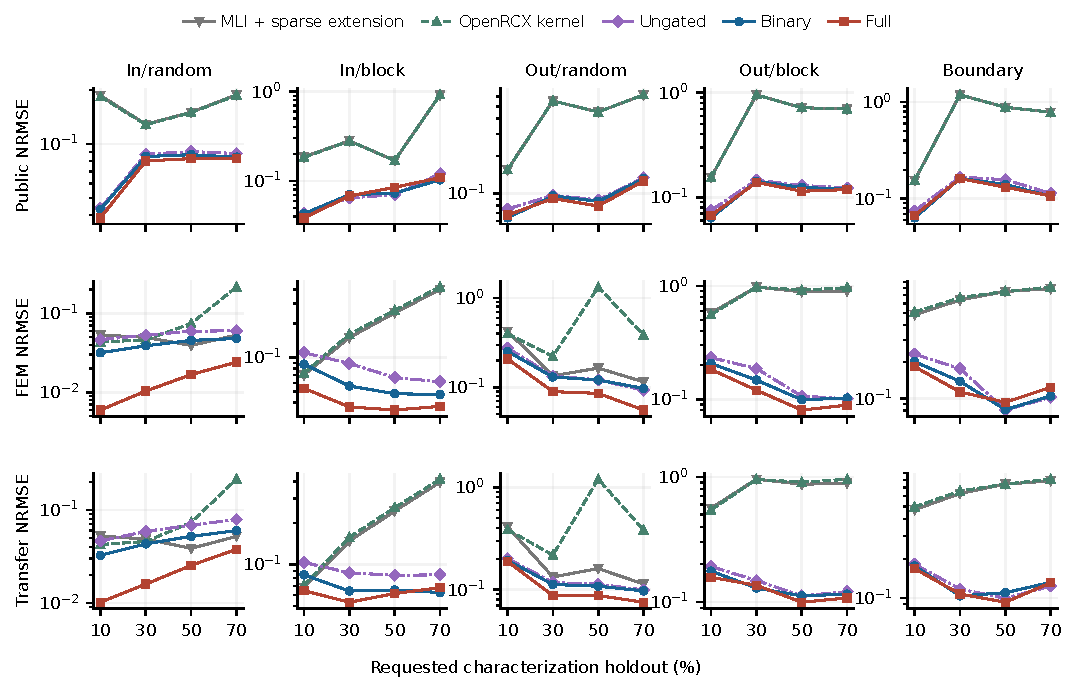
\includegraphics[width=\textwidth]{figures/coverage_four_ratios.pdf}
\caption{All four characterization holdouts on common feasible S/Q. Complete-cell and sparse-support-extension coverage is recorded independently of errors.}\label{fig:coverage}\end{figure*}
\begin{table*}[t]\centering\caption{Public rules: complete four-holdout sensitivity, mean-mask macro NRMSE. MLI-ext. includes declared sparse/boundary extensions; ORCX includes native mapping and quantization. Selected GP is source-validation-frozen.}\small\begin{tabular}{llrrrrrr}
\toprule
Condition & Holdout\% & ORCX & MLI-ext. & Anchor & Sel. GP & Binary & Full \\
\midrule
In/random & 10 & 0.1835 & 0.1862 & 0.1862 & 0.1363 & 0.0430 & 0.0386 \\
In/random & 30 & 0.1279 & 0.1286 & 0.1286 & 0.1520 & 0.0850 & 0.0803 \\
In/random & 50 & 0.1496 & 0.1502 & 0.1502 & 0.1742 & 0.0870 & 0.0827 \\
In/random & 70 & 0.1865 & 0.1879 & 0.1879 & 0.1994 & 0.0843 & 0.0827 \\
In/block & 10 & 0.1835 & 0.1862 & 0.1862 & 0.1363 & 0.0430 & 0.0386 \\
In/block & 30 & 0.2806 & 0.2812 & 0.2812 & 0.2370 & 0.0701 & 0.0678 \\
In/block & 50 & 0.1693 & 0.1692 & 0.1692 & 0.1771 & 0.0731 & 0.0849 \\
In/block & 70 & 0.9212 & 0.9221 & 0.9221 & 0.8324 & 0.1029 & 0.1089 \\
Out/random & 10 & 0.1550 & 0.1550 & 0.1550 & 0.5119 & 0.0636 & 0.0670 \\
Out/random & 30 & 0.5531 & 0.5531 & 0.5531 & 0.5563 & 0.0954 & 0.0910 \\
Out/random & 50 & 0.4511 & 0.4511 & 0.4511 & 0.4984 & 0.0864 & 0.0792 \\
Out/random & 70 & 0.6195 & 0.6195 & 0.6195 & 0.6775 & 0.1313 & 0.1259 \\
Out/block & 10 & 0.1550 & 0.1550 & 0.1550 & 0.5119 & 0.0636 & 0.0670 \\
Out/block & 30 & 0.9546 & 0.9546 & 0.9546 & 1.7986 & 0.1420 & 0.1391 \\
Out/block & 50 & 0.7181 & 0.7181 & 0.7181 & 1.3788 & 0.1242 & 0.1143 \\
Out/block & 70 & 0.6984 & 0.6984 & 0.6984 & 1.0038 & 0.1197 & 0.1186 \\
Boundary & 10 & 0.1550 & 0.1550 & 0.1550 & 0.5119 & 0.0636 & 0.0670 \\
Boundary & 30 & 1.1867 & 1.1867 & 1.1867 & 2.4125 & 0.1629 & 0.1620 \\
Boundary & 50 & 0.8819 & 0.8819 & 0.8819 & 2.1336 & 0.1404 & 0.1319 \\
Boundary & 70 & 0.7849 & 0.7849 & 0.7849 & 1.3501 & 0.1066 & 0.1073 \\
\bottomrule
\end{tabular}
\end{table*}
\begin{table*}[t]\centering\caption{FEM: complete four-holdout sensitivity, mean-mask macro NRMSE. MLI-ext. includes declared sparse/boundary extensions; ORCX includes native mapping and quantization. Selected GP is source-validation-frozen.}\small\begin{tabular}{llrrrrrr}
\toprule
Condition & Holdout\% & ORCX & MLI-ext. & Anchor & Sel. GP & Binary & Full \\
\midrule
In/random & 10 & 0.0431 & 0.0531 & 0.0127 & 0.0260 & 0.0315 & 0.0059 \\
In/random & 30 & 0.0461 & 0.0495 & 0.0208 & 0.0261 & 0.0387 & 0.0103 \\
In/random & 50 & 0.0739 & 0.0391 & 0.0328 & 0.0278 & 0.0453 & 0.0167 \\
In/random & 70 & 0.2150 & 0.0528 & 0.0577 & 0.0307 & 0.0479 & 0.0240 \\
In/block & 10 & 0.0729 & 0.0703 & 0.0669 & 0.1211 & 0.0874 & 0.0534 \\
In/block & 30 & 0.1604 & 0.1502 & 0.1286 & 0.1415 & 0.0560 & 0.0366 \\
In/block & 50 & 0.2624 & 0.2481 & 0.2281 & 0.8488 & 0.0479 & 0.0343 \\
In/block & 70 & 0.4204 & 0.4008 & 0.3332 & 0.9599 & 0.0471 & 0.0370 \\
Out/random & 10 & 0.3968 & 0.4236 & 0.0421 & 12.6661 & 0.2525 & 0.2077 \\
Out/random & 30 & 0.2220 & 0.1344 & 0.0606 & 0.0742 & 0.1303 & 0.0895 \\
Out/random & 50 & 1.3237 & 0.1639 & 0.1818 & 2.8463 & 0.1207 & 0.0855 \\
Out/random & 70 & 0.3837 & 0.1151 & 0.2004 & 0.2486 & 0.0972 & 0.0557 \\
Out/block & 10 & 0.5587 & 0.5769 & 0.3737 & 4.6219 & 0.2066 & 0.1832 \\
Out/block & 30 & 0.9767 & 0.9790 & 0.6542 & 0.3698 & 0.1479 & 0.1203 \\
Out/block & 50 & 0.9202 & 0.8870 & 0.6301 & 2.5131 & 0.0991 & 0.0803 \\
Out/block & 70 & 0.9653 & 0.9009 & 0.7142 & 7.5279 & 0.1025 & 0.0887 \\
Boundary & 10 & 0.5101 & 0.4857 & 0.4429 & 50.3460 & 0.2007 & 0.1826 \\
Boundary & 30 & 0.6691 & 0.6404 & 0.5663 & 21.3179 & 0.1388 & 0.1137 \\
Boundary & 50 & 0.7525 & 0.7525 & 0.7525 & 4.7971 & 0.0814 & 0.0935 \\
Boundary & 70 & 0.8182 & 0.7935 & 0.7694 & 1.3120 & 0.1053 & 0.1239 \\
\bottomrule
\end{tabular}
\end{table*}
\begin{table*}[t]\centering\caption{Transfer: complete four-holdout sensitivity, mean-mask macro NRMSE. MLI-ext. includes declared sparse/boundary extensions; ORCX includes native mapping and quantization. Selected GP is source-validation-frozen.}\small\begin{tabular}{llrrrrrr}
\toprule
Condition & Holdout\% & ORCX & MLI-ext. & Anchor & Sel. GP & Binary & Full \\
\midrule
In/random & 10 & 0.0425 & 0.0523 & 0.0125 & 0.0252 & 0.0325 & 0.0102 \\
In/random & 30 & 0.0458 & 0.0488 & 0.0205 & 0.0252 & 0.0432 & 0.0159 \\
In/random & 50 & 0.0735 & 0.0386 & 0.0321 & 0.0269 & 0.0520 & 0.0254 \\
In/random & 70 & 0.2142 & 0.0520 & 0.0565 & 0.0297 & 0.0600 & 0.0378 \\
In/block & 10 & 0.0704 & 0.0679 & 0.0641 & 0.1178 & 0.0838 & 0.0643 \\
In/block & 30 & 0.1575 & 0.1473 & 0.1246 & 0.1379 & 0.0640 & 0.0531 \\
In/block & 50 & 0.2580 & 0.2439 & 0.2223 & 0.7915 & 0.0651 & 0.0614 \\
In/block & 70 & 0.4149 & 0.3949 & 0.3262 & 0.9178 & 0.0624 & 0.0678 \\
Out/random & 10 & 0.3857 & 0.4122 & 0.0413 & 9.6995 & 0.1933 & 0.1886 \\
Out/random & 30 & 0.2173 & 0.1330 & 0.0595 & 0.0724 & 0.1124 & 0.0877 \\
Out/random & 50 & 1.1965 & 0.1607 & 0.1787 & 2.2440 & 0.1080 & 0.0876 \\
Out/random & 70 & 0.3810 & 0.1133 & 0.1978 & 0.2281 & 0.0973 & 0.0754 \\
Out/block & 10 & 0.5444 & 0.5614 & 0.3625 & 3.6935 & 0.1764 & 0.1574 \\
Out/block & 30 & 0.9562 & 0.9583 & 0.6374 & 0.3636 & 0.1291 & 0.1358 \\
Out/block & 50 & 0.9062 & 0.8729 & 0.6183 & 2.3093 & 0.1117 & 0.0994 \\
Out/block & 70 & 0.9562 & 0.8914 & 0.7054 & 7.1295 & 0.1155 & 0.1077 \\
Boundary & 10 & 0.4974 & 0.4737 & 0.4322 & 39.8743 & 0.1759 & 0.1677 \\
Boundary & 30 & 0.6574 & 0.6297 & 0.5580 & 18.6305 & 0.1037 & 0.1073 \\
Boundary & 50 & 0.7429 & 0.7429 & 0.7429 & 4.4843 & 0.1099 & 0.0929 \\
Boundary & 70 & 0.8100 & 0.7862 & 0.7629 & 1.2832 & 0.1317 & 0.1308 \\
\bottomrule
\end{tabular}
\end{table*}

\subsection{Same-physics kernel and generated-table evaluation}
Table~\ref{tab:production} drives both production-related kernels with the same FEM-characterized samples. Specified MLI obtains NRMSE 0.00452; the mapped/quantized OpenRCX kernel obtains 0.01072. Its ideal continuous-distance counterpart obtains 0.00635, isolating one implementation effect without introducing width interpolation. Full/Binary values retrieved through populated compute tables obtain 0.02447/0.02901. Full does not improve over the native kernel on this complete-support cohort. These values use a complete-slot preparation protocol and native mapping, so direct-query errors cannot be substituted for them. Extracted pinned function bodies agree with the Python evaluator, and native-value pass-through preserves the kernel outputs.

\begin{table*}[t]
\begin{minipage}[t]{.48\textwidth}
\centering\caption{Production-related kernel evaluation on the same 71 independently referenced templates.}\label{tab:production}\small\begin{tabular}{lrr}
\toprule
Method & NRMSE & P95 (pF/m) \\
\midrule
OpenRCX kernel & 0.01072 & 0.799 \\
Specified MLI & 0.00452 & 0.240 \\
Binary & 0.02218 & 1.337 \\
Full & 0.01675 & 1.024 \\
Binary compute table & 0.02901 & 1.473 \\
Full compute table & 0.02447 & 1.554 \\
\bottomrule
\end{tabular}

\end{minipage}\hfill
\begin{minipage}[t]{.48\textwidth}
\centering\caption{Full-support numerical and conditional controls; reused warm runtime.}\label{tab:components}\small\begin{tabular}{lrr}
\toprule
Control & NRMSE & Warm ms/Q \\
\midrule
Anchor & 0.00451 & 0.788 \\
CMI extension & 0.00452 & 0.923 \\
Selected GP & 0.05371 & 0.316 \\
Local affine & 0.05254 & 0.232 \\
Ungated & 0.02688 & 2.051 \\
Binary & 0.02218 & 2.110 \\
Full & 0.01675 & 3.706 \\
Adapted MLP & 0.01889 & 0.025 \\
CNP & 0.16575 & 0.155 \\
Adapted AC & 0.70695 & 0.230 \\
\bottomrule
\end{tabular}

\end{minipage}
\par\bigskip
\centering\caption{New Full compute-table deployment: net-C fidelity, mean extraction ratio and cold preparation/PEX/SPEF wall seconds.}\label{tab:deployment}\small\begin{tabular}{lrrrrr}
\toprule
Layout & C err. & Prep. & PEX & SPEF & $T/T_0$ \\
\midrule
asap7/aes & 0.00426 & 5.41 & 2.05 & 0.49 & 0.991 \\
asap7/ibex & 0.00516 & 5.41 & 3.30 & 0.72 & 1.020 \\
gf180/aes & 0.00030 & 8.39 & 2.45 & 0.52 & 1.031 \\
gf180/ibex & 0.00020 & 8.39 & 2.73 & 0.52 & 0.999 \\
IHP/aes & 0.05656 & 13.99 & 2.00 & 0.40 & 1.035 \\
IHP/ibex & 0.05477 & 13.99 & 3.10 & 0.66 & 1.029 \\
Sky/aes & 0.00382 & 8.48 & 2.43 & 0.56 & 1.017 \\
Sky/ibex & 0.00233 & 8.48 & 2.29 & 0.58 & 1.024 \\
\bottomrule
\end{tabular}

\end{table*}

The scalar projection wrapper does not claim equivalence between native calibration materials and the FEM stack. Its third output channel carries the declared diagonal template projection; it is not a native resistance measurement. Rank-four MLI is tested on known multilinear functions only. The production injection retains native resistance without using that scalar wrapper.
% Balance the two columns of the production-results discussion.
\newpage
\subsection{New computeTable measurements}
The full-characterization interface populates 49,657 eligible finite slots across four rule libraries. Native-value pass-through preserves traced getter returns and electrical SPEF records on all eight layouts. Full changes 924,647 traced returns; covered returns match injected values, and resistance/uncovered returns remain identical. Table~\ref{tab:deployment} reports this archived full-characterization path: across 120 release runs, the Full extraction/original ratio ranges from 0.991 to 1.035. Summing archived inventory, input/model/support preparation and native-process startup residual, modeled first-design PEX overhead ranges from 161.1\% to 670.4\%. SPEF output and STA are measured separately and are not used to dilute this denominator. Values below one are repeat-run variation, not a stable acceleration claim.


The new release build leaves getters unchanged. The preparation hook updates coupling/fringe only after native table construction; a separate trace build validates every covered return. Entire special-tail and diagonal tables remain native, as do measurement-bin conflicts and direct measure-table boundary returns. Inventories from both designs match within each process. The cache therefore enumerates the supported rule grid, rather than just the current design's requested slots.

Cold preparation charges the inventory extraction required by the pinned deferred-loading API, model loading, support mapping, inference and payload output. Full-model bundle loading is not claimed free for the first design. Per-process cold totals charge a complete load; the two-design reuse accounting charges it once per prepared library. Process residual is total wall minus named Tcl stages and includes startup/payload loading and shutdown, not an isolated parse benchmark. Native compute construction and hook application are measured within extraction. The detailed CSV separates these boundaries, PEX-only overhead, SPEF and STA; source training is separately reported and no training is repeated.


\begin{table*}[t]\centering\caption{Supplied model cost: sum of three members' recorded final-stage training wall seconds, not parallel elapsed. Hardware and source-training opportunity differ; these are provenance costs, not matched speed rankings. Missing receipts are shown as --. Initialization, source-label generation and model selection are not fully aggregated, so complete training cost is unavailable.}\label{tab:sourcecost}\small\begin{tabular}{lrrrrrr}
\toprule
Setting & Full & Binary & Ungated & MLP & CNP & Adapted AC \\
\midrule
Public & 2377.3 & 4629.3 & 4328.5 & 16.9 & 26.3 & -- \\
FEM & -- & -- & -- & -- & -- & -- \\
Transfer & 5005.4 & 5797.1 & 5720.7 & 18.9 & 29.8 & 51.2 \\
\bottomrule
\end{tabular}
\end{table*}
The common 918 physical support geometries have recorded fine-solver CPU cost 4,889.83\,s, or 11,761.63\,s for three-level certification. These supplied-input costs are not charged per query and are not new computation. Public rule characterization cost is unavailable.
\begin{table*}[t]\centering\caption{Complete new compute-table pipeline: three runs per layout/mode. PEX, its sample SD, SPEF output, STA read/analysis and external cold preparation are wall seconds. Net-C error and slack difference use the original full-rule reference. Preparation is reusable within a process library; native table construction/injection remains inside PEX.}\label{tab:allstages}\small\begin{tabular}{llrrrrrrr}
\toprule
Layout & Mode & PEX & SD & SPEF & STA & Prep. & C err. & $\Delta$slack (ps) \\
\midrule
asap7/aes & original & 2.071 & 0.044 & 0.553 & 3.429 & 0 & 0 & 0 \\
asap7/aes & disabled & 2.049 & 0.028 & 0.485 & 3.548 & 0.00 & 0.00000 & +0.000 \\
asap7/aes & pass & 2.056 & 0.020 & 0.483 & 3.638 & 4.45 & 0.00000 & +0.000 \\
asap7/aes & binary & 2.045 & 0.018 & 0.532 & 3.529 & 5.08 & 0.00568 & +0.213 \\
asap7/aes & full & 2.053 & 0.007 & 0.489 & 3.442 & 5.41 & 0.00426 & +0.173 \\
asap7/ibex & original & 3.240 & 0.026 & 0.711 & 5.624 & 0 & 0 & 0 \\
asap7/ibex & disabled & 3.274 & 0.011 & 0.720 & 5.669 & 0.00 & 0.00000 & +0.000 \\
asap7/ibex & pass & 3.362 & 0.068 & 0.771 & 5.688 & 4.45 & 0.00000 & +0.000 \\
asap7/ibex & binary & 3.259 & 0.014 & 0.723 & 5.883 & 5.08 & 0.00675 & +0.644 \\
asap7/ibex & full & 3.305 & 0.055 & 0.721 & 5.655 & 5.41 & 0.00516 & +0.510 \\
gf180/aes & original & 2.376 & 0.024 & 0.510 & 3.128 & 0 & 0 & 0 \\
gf180/aes & disabled & 2.437 & 0.028 & 0.550 & 3.109 & 0.00 & 0.00000 & +0.000 \\
gf180/aes & pass & 2.415 & 0.013 & 0.529 & 3.152 & 4.42 & 0.00000 & +0.000 \\
gf180/aes & binary & 2.418 & 0.018 & 0.531 & 3.233 & 6.62 & 0.00096 & +0.723 \\
gf180/aes & full & 2.449 & 0.002 & 0.523 & 3.252 & 8.39 & 0.00030 & +0.168 \\
gf180/ibex & original & 2.736 & 0.068 & 0.516 & 4.102 & 0 & 0 & 0 \\
gf180/ibex & disabled & 2.687 & 0.100 & 0.520 & 4.097 & 0.00 & 0.00000 & +0.000 \\
gf180/ibex & pass & 2.717 & 0.144 & 0.509 & 4.066 & 4.42 & 0.00000 & +0.000 \\
gf180/ibex & binary & 2.654 & 0.015 & 0.514 & 4.009 & 6.62 & 0.00086 & +1.522 \\
gf180/ibex & full & 2.733 & 0.042 & 0.515 & 4.202 & 8.39 & 0.00020 & +0.205 \\
IHP/aes & original & 1.934 & 0.004 & 0.446 & 2.831 & 0 & 0 & 0 \\
IHP/aes & disabled & 1.914 & 0.025 & 0.390 & 2.879 & 0.00 & 0.00000 & +0.000 \\
IHP/aes & pass & 2.011 & 0.018 & 0.407 & 2.855 & 4.58 & 0.00000 & +0.000 \\
IHP/aes & binary & 2.070 & 0.128 & 0.418 & 2.871 & 9.60 & 0.05926 & +78.138 \\
IHP/aes & full & 2.003 & 0.070 & 0.401 & 2.849 & 13.99 & 0.05656 & +74.414 \\
IHP/ibex & original & 3.008 & 0.062 & 0.610 & 4.122 & 0 & 0 & 0 \\
IHP/ibex & disabled & 2.994 & 0.044 & 0.590 & 4.157 & 0.00 & 0.00000 & +0.000 \\
IHP/ibex & pass & 3.276 & 0.301 & 0.600 & 4.129 & 4.58 & 0.00000 & +0.000 \\
IHP/ibex & binary & 3.068 & 0.014 & 0.657 & 4.093 & 9.60 & 0.05742 & +154.548 \\
IHP/ibex & full & 3.095 & 0.055 & 0.661 & 4.137 & 13.99 & 0.05477 & +147.439 \\
Sky/aes & original & 2.387 & 0.022 & 0.502 & 3.655 & 0 & 0 & 0 \\
Sky/aes & disabled & 2.429 & 0.044 & 0.516 & 3.610 & 0.00 & 0.00000 & +0.000 \\
Sky/aes & pass & 2.454 & 0.019 & 0.580 & 3.696 & 5.07 & 0.00000 & +0.000 \\
Sky/aes & binary & 2.414 & 0.037 & 0.508 & 3.782 & 7.01 & 0.01154 & +6.319 \\
Sky/aes & full & 2.426 & 0.046 & 0.559 & 3.595 & 8.48 & 0.00382 & +2.276 \\
Sky/ibex & original & 2.238 & 0.011 & 0.499 & 4.064 & 0 & 0 & 0 \\
Sky/ibex & disabled & 2.275 & 0.063 & 0.470 & 4.119 & 0.00 & 0.00000 & +0.000 \\
Sky/ibex & pass & 2.269 & 0.011 & 0.468 & 4.060 & 5.07 & 0.00000 & +0.000 \\
Sky/ibex & binary & 2.300 & 0.020 & 0.485 & 4.099 & 7.01 & 0.01065 & +11.272 \\
Sky/ibex & full & 2.292 & 0.057 & 0.584 & 4.046 & 8.48 & 0.00233 & +2.392 \\
\bottomrule
\end{tabular}
\end{table*}

\clearpage
\raggedbottom
\section{Conclusion}
We presented characterization-conditioned capacitance estimation with an anchor-based residual predictor, binary and numerical--neural gates, and internal compute-table population as well as native rule export. Experiments connect completion to extraction and timing fidelity, showing how support coverage, target adaptation, and fusion complexity affect accuracy and cost. The native census establishes the occurrence of non-node requests, while direct template references show that learned corrections need not improve interpolation when the full characterization support is available. Support conditions and physical interface coverage determine the useful scope of conditional estimation.


\bibliographystyle{IEEEtran}
\bibliography{references}
\end{document}
